\documentclass[conference,10pt]{IEEEtran}
\IEEEoverridecommandlockouts
\PassOptionsToPackage{table}{xcolor}
\usepackage[T1]{fontenc}
\usepackage{mathptmx}
\usepackage{graphicx}
\usepackage{booktabs}
\usepackage{multirow}
\usepackage{amsmath}
\usepackage{algorithm}
\usepackage{algpseudocode}
\usepackage{tikz}
\usetikzlibrary{positioning,fit,arrows.meta,calc}
\usepackage{xcolor}
\usepackage[hyphens]{url}
\usepackage[hidelinks]{hyperref}
\usepackage{tabularx}
\usepackage{array}
\usepackage{balance}

\newcommand{\krps}{k\,req/s}
\newcommand{\us}{\,\textmu s}
\newcommand{\code}[1]{\texttt{#1}}
\renewcommand{\arraystretch}{1.08}
\setlength{\tabcolsep}{3.6pt}

\begin{document}

\title{Scalable Network I/O: From select to io\_uring\\
\large CS331 Computer Networks \textbar{} Team T016 \textbar{} Project ID 13}

\author{%
\begin{tabular}{@{}c@{\hspace{12mm}}c@{\hspace{12mm}}c@{}}
Kale Parth Hemant & Devvrat Hans & Patil Nachiket Kiran\\
\textit{\small 24110242} & \textit{\small 23110094} & \textit{\small 24110250}\\[3mm]
Niraj Kumar & Chirag Agarwalla & Nityanand Karmali\\
\textit{\small 24110222} & \textit{\small 24110093} & \textit{\small 24110226}
\end{tabular}}

\maketitle


%======================================================================
\section{Introduction}
Chat servers, file servers, video relays and key-value stores all keep many network connections open at once. Giving each connection its own thread wastes memory and causes scheduler overhead, so most servers use an \emph{event loop}: one thread asks the kernel which sockets are ready, serves those, and asks again. How the thread asks is the I/O multiplexing mechanism, and its cost is paid on every request.

Linux has four generations of this mechanism. \code{select} (1983) and \code{poll} (1986) pass the full list of interesting descriptors on every call, so the kernel scans all of them. \code{epoll} (2002) registers interest once and returns only ready descriptors. \code{io\_uring} (2019) changes the model: the application submits whole operations (accept, receive, send) to a ring in shared memory and later reads their completions, so one system call can carry many operations, or none at all.

The common wisdom is ``\code{epoll} scales, \code{select} does not, \code{io\_uring} is fastest''. Published measurements are more mixed [3], [7], and the answer depends on the workload. This project measures \emph{when} each mechanism is better and explains \emph{why} in operating-system terms.

\textbf{Contributions.}
(1) A plugin framework that runs six applications, over TCP and UDP, on four interchangeable engines that share all other code, so the engines are the only variable.
(2) A measurement method with exact in-server system-call counters (checked against \code{strace}), per-core interrupt and softirq accounting, run-queue wait, and closed-loop and paced load that avoids coordinated omission.
(3) 18 experiment suites (1140 valid runs) that vary connections, idle descriptors, message size, transfer direction, transport, offered load, buffer size and thread count, plus the extensions the TA asked for: level- versus edge-triggered \code{epoll}, \code{io\_uring} SQPOLL, and multithreaded servers.
(4) An explanation of each result in terms of system calls, scanning, wakeups, interrupts, CPU and memory.

In short, no mechanism wins everywhere. With every connection busy, \code{select} and \code{poll} match or beat default \code{epoll}, which pays two \code{epoll\_ctl} calls per request. With idle connections, \code{select} and \code{poll} lose 78\% of their throughput between 10 and 1000 descriptors while \code{epoll} and \code{io\_uring} stay flat. \code{io\_uring} gives 6--15\% more throughput when batching is possible and nothing when it is not, and its CPU use follows the offered load; only the SQPOLL mode keeps a core busy at every load.

%======================================================================
\section{Problem Statement}
\textbf{Problem.} Given a single-threaded server on Linux, determine how the choice of I/O multiplexing mechanism affects throughput, latency, CPU cost and kernel activity, and how that answer changes with the application and the load.

\textbf{Inputs (independent variables):} mechanism (\code{select}, \code{poll}, \code{epoll} in three modes, \code{io\_uring} in three modes); application (noop, echo, upload, download, stream, memory); transport (TCP, UDP); number of connections (1--1000) and how many are idle; message size (1\,B--1\,MiB); arrival model (closed loop, or a fixed paced rate of 1k--40k\,req/s); server buffer size (4--64\,KiB); number of event-loop threads (1, 2, 4).

\textbf{Outputs (measured):} verified requests per second, payload MiB/s, latency p50/p99/p99.9, server CPU (user and kernel), CPU time per request, system calls per message by type, voluntary context switches (wakeups), network softirqs and hardware interrupts on the server core, run-queue wait, and peak resident memory.

\textbf{Assumptions and constraints.} One machine, loopback networking (to isolate the software cost of each mechanism from a network card), non-blocking sockets, and an unmodified Ubuntu kernel. The client must never be the bottleneck, and every run must pass a correctness check.

\textbf{In scope:} event-loop servers with one or more independent loops. \textbf{Out of scope:} thread-per-connection servers, real NICs and RDMA, kernel bypass (DPDK), storage I/O, and \code{io\_uring} multishot receive (not available in liburing 2.1).

\textbf{Gap.} Earlier studies compared \code{select}, \code{poll} and \code{epoll} on one web workload [3], or \code{io\_uring} on storage [6]. Our first version also compared the engines on a single echo benchmark, which cannot show that the best mechanism depends on the application. A fair comparison needs the same application code on every engine, several application types, and an explanation from the OS side, which is what this project provides.

%======================================================================
\section{Project Objectives}
\begin{enumerate}
\item Build the framework first: a shared core (sockets, request state machine, UDP, threads, signals, statistics) and a plugin interface, so any application runs on any engine over TCP or UDP.
\item Implement four engines that contain \emph{only} their event loop: \code{select}, \code{poll}, \code{epoll} (level-triggered, edge-triggered, level-triggered with immediate reply) and \code{io\_uring} (plain, SQPOLL, SQPOLL with busy completion polling).
\item Provide a no-op baseline in which the loop does no useful work, giving each engine's top request frequency.
\item Measure latency-sensitive, read-heavy, write-heavy, streaming and memory-heavy applications, over TCP and UDP, with 1 to 1000 descriptors.
\item Answer the TA's question on \code{io\_uring} CPU use by measuring CPU against a controlled offered load.
\item Record wakeups, interrupts and softirqs, explain every difference from the OS point of view, and check every measurement for correctness.
\end{enumerate}

%======================================================================
\section{Background and Related Work}
\textbf{Readiness versus completion.} \code{select}, \code{poll} and \code{epoll} report \emph{readiness}: the kernel says a socket can be read or written without blocking, and the program then calls \code{recv} or \code{send}. \code{io\_uring} reports \emph{completion}: the program hands the kernel a \code{recv} with a buffer, and later reads a completion entry stating how many bytes arrived.

\textbf{Cost per call.} \code{select} copies three bitmaps of up to 1024 bits (\code{FD\_SETSIZE}) into the kernel; the kernel calls each socket's \code{poll} method, adds the thread to each socket's wait queue, sleeps, and on wakeup scans every descriptor again because it does not know which one woke it. \code{poll} replaces the bitmaps with an array of \code{struct pollfd}, which removes the 1024 limit but keeps the $O(N)$ scan. \code{epoll} keeps an interest set in the kernel: sockets that become ready put themselves on a ready list through a callback, so \code{epoll\_wait} costs $O(\text{ready})$. Changing interest (for example, from reading to writing) costs an \code{epoll\_ctl} system call. In level-triggered (LT) mode a ready socket is reported again on every wait; in edge-triggered (ET) mode only when its state changes, so the program must read or write until \code{EAGAIN}.

\code{io\_uring} shares a submission queue (SQ) and a completion queue (CQ) with the kernel. One \code{io\_uring\_enter} call can submit many operations and wait for completions; if completions are already in the CQ, no system call is needed at all. With SQPOLL, a kernel thread polls the SQ, so the application does not need to make system calls to submit either, at the cost of a thread that spins while there is work and sleeps after an idle timeout.

\textbf{Related work.} Banga, Mogul and Druschel showed that \code{select} scales poorly as descriptors grow and proposed registering interest once, the idea behind \code{epoll} [1]. Provos and Lever made \code{poll} cheaper with \code{/dev/poll} and compared it with POSIX real-time signals [2]. Gammo et al.\ found \code{select} and \code{poll} comparable to \code{epoll} when there are no idle connections, and attributed part of \code{epoll}'s cost to \code{epoll\_ctl} [3]. FlexSC showed the benefit of batching system calls through shared memory [4], the idea \code{io\_uring} builds on [8]. Schroeder et al.\ showed that closed and open load generators can lead to different conclusions [5], which motivated our paced mode. Didona et al.\ studied \code{io\_uring} polling modes for storage [6], and a recent DBMS study found that replacing \code{epoll} with \code{io\_uring} gave about 1.1$\times$ for network traffic, with SQPOLL worthwhile only when a dedicated core is justified [7]. These papers predict that (a) with all connections active the readiness mechanisms are close, (b) with idle connections \code{select}/\code{poll} degrade and \code{epoll} does not, and (c) \code{io\_uring} gives a modest gain. We test these predictions on six applications and over UDP.

%======================================================================
\section{Architecture and Design}
\begin{figure}[t]
\centering
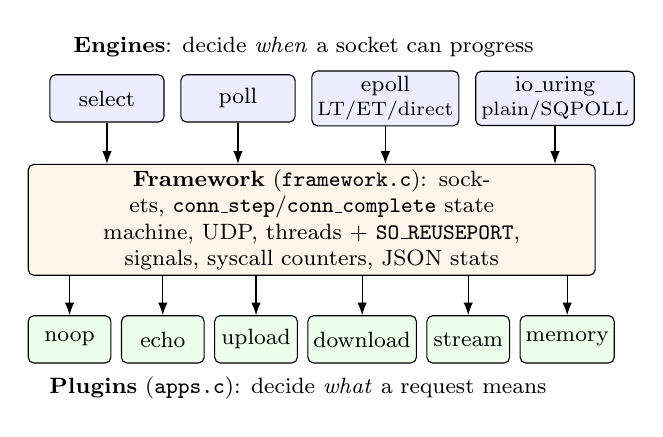
\begin{tikzpicture}[font=\footnotesize, node distance=2mm,
  box/.style={draw, rounded corners=2pt, align=center, minimum height=6mm, inner sep=2pt},
  eng/.style={box, fill=blue!7, minimum width=14.5mm},
  fw/.style={box, fill=orange!8},
  app/.style={box, fill=green!8, minimum width=10.5mm}]
\node[eng] (s) {select};
\node[eng, right=of s] (p) {poll};
\node[eng, right=of p] (e) {epoll\\[-1pt]\scriptsize LT/ET/direct};
\node[eng, right=of e] (u) {io\_uring\\[-1pt]\scriptsize plain/SQPOLL};
\node[above=1mm of p.north east, anchor=south, xshift=1mm] {\textbf{Engines}: decide \emph{when} a socket can progress};
\node[fw, below=5mm of $(p.south)!0.5!(e.south)$, minimum width=72mm, text width=70mm] (fw) {\textbf{Framework} (\code{framework.c}): sockets, \code{conn\_step}/\code{conn\_complete} state\\machine, UDP, threads + \code{SO\_REUSEPORT}, signals, syscall counters, JSON stats};
\node[app, below=5mm of fw.south west, anchor=north west] (a1) {noop};
\node[app, right=1.2mm of a1] (a2) {echo};
\node[app, right=1.2mm of a2] (a3) {upload};
\node[app, right=1.2mm of a3] (a4) {download};
\node[app, right=1.2mm of a4] (a5) {stream};
\node[app, right=1.2mm of a5] (a6) {memory};
\node[below=0.5mm of a3.south east, anchor=north] {\textbf{Plugins} (\code{apps.c}): decide \emph{what} a request means};
\foreach \n in {s,p,e,u} \draw[-{Latex[length=1.6mm]}] (\n.south) -- (\n.south |- fw.north);
\foreach \n in {a1,a2,a3,a4,a5,a6} \draw[{Latex[length=1.6mm]}-] (\n.north) -- (\n.north |- fw.south);
\end{tikzpicture}
\caption{Three layers. Every engine implements one function, \code{engine\_run}; every plugin implements the \code{app\_ops\_t} callbacks. The framework and plugins are compiled once and linked into all four servers. The C load generator connects over loopback.}
\label{fig:arch}
\end{figure}

Fig.~\ref{fig:arch} shows the three layers. An engine never looks at an application and an application never makes a socket call, so any plugin runs on any engine over TCP or UDP.

\textbf{Plugin contract.} A plugin provides \code{validate(length)}, \code{body\_size} and \code{response\_size} (bytes in and out), \code{on\_body} (consume received bytes), \code{fill} (produce reply bytes), \code{on\_open}/\code{on\_close} (per-client state) and \code{on\_datagram} (the same application as one UDP datagram). The six plugins are: \textbf{noop}, an 8-byte header answered with one byte (the baseline where the loop does no useful work); \textbf{echo}, a latency-sensitive chat-like exchange; \textbf{upload}, a read-heavy transfer in which every byte is verified; \textbf{download}, a write-heavy transfer of a known byte pattern; \textbf{stream}, 64\,KiB frames paced by the client like video; and \textbf{memory}, in which every client owns a resident 256\,KiB buffer that each request writes into.

\textbf{Wire format.} A TCP request is an 8-byte big-endian length followed by the body; the reply length is set by the plugin. A UDP datagram carries an 8-byte sequence number, the requested reply length and the body, since UDP keeps message boundaries.

\textbf{Shared request state machine.} Each client is a \code{conn\_t} with a stage (\code{HEADER}, \code{RECEIVE}, \code{SEND}), progress counters \code{done}/\code{want}, and a buffer (4\,KiB by default). \code{conn\_step} performs exactly one \code{recv} or \code{send}, whichever the stage needs, and passes the result to \code{conn\_complete}, which advances the state. \code{io\_uring} calls \code{conn\_complete} directly with the result from a completion entry, so all four engines share the same state machine and partial reads and writes are handled once. A client never has a read and a write in flight together, so one buffer per client is safe.

\textbf{Key design decisions.}
\emph{(a) Shared code instead of one copy per engine.} In our first version each server had its own copy of the application code; GCC compiled a per-byte check differently in each, and that alone made two engines look 60\% faster on upload. Compiling the framework and plugins once removed this bias.
\emph{(b) Counting system calls inside the server.} \code{strace} slows a server several times and changes its batching, so the servers count every I/O system call themselves; we validated the counters against \code{strace -c}.
\emph{(c) Loopback.} It removes NIC and wire effects so the measured differences are the mechanisms' own. The trade-off is that the receiver's network processing (the NET\_RX softirq) runs on the sending CPU, which we account for explicitly.
\emph{(d) Independent loops for threads.} Each thread has its own listening socket with \code{SO\_REUSEPORT}, so the kernel spreads connections and no lock is ever taken. A shared-queue design would have measured lock contention instead of the mechanisms.
\emph{(e) Signals.} \code{SIGINT}/\code{SIGTERM} handlers only set a flag (handlers may call only async-signal-safe functions); waits are not restarted (\code{SA\_RESTART} unset) and time out every 100\,ms, so the loop notices the flag. \code{SIGPIPE} is ignored and sends use \code{MSG\_NOSIGNAL}, so a closed client gives \code{EPIPE} instead of killing the server.

%======================================================================
\section{Implementation}
The servers, framework and load generator are written in C11 (about 2{,}500 lines) and built with \code{gcc -O2 -Wall -Wextra -Werror}; \code{io\_uring} uses liburing 2.1. The experiment runner and analysis are in Python 3. The code is at \url{https://github.com/devvrat-hans/CS331-T016-ScalableNetworkIO}.

\textbf{select} keeps a table of clients indexed by descriptor, rebuilds the read/write sets before each call (the kernel overwrites them), and walks descriptors up to the highest one. A descriptor $\geq$ \code{FD\_SETSIZE} cannot be represented and is rejected cleanly. \textbf{poll} keeps a parallel \code{pollfd[]}/\code{clients[]} array with the listener in slot~0 and rebuilds interest each iteration. \textbf{epoll} registers each client once; in LT mode it switches interest between \code{EPOLLIN} and \code{EPOLLOUT} with \code{EPOLL\_CTL\_MOD} (two \code{epoll\_ctl} calls per request); \emph{LT-direct} tries the reply immediately and arms \code{EPOLLOUT} only if the send would block; ET registers \code{EPOLLIN|EPOLLOUT|EPOLLET} once and reads or writes until \code{EAGAIN}. Algorithm~\ref{alg:uring} shows the \textbf{io\_uring} loop.

\begin{algorithm}[t]
\caption{io\_uring event loop (one thread)}\label{alg:uring}
\small
\begin{algorithmic}[1]
\State set up ring: SQ depth 256, CQ sized for all clients (\code{IORING\_SETUP\_CQSIZE}); optional \code{SQPOLL} pinned to its own core
\State queue one \code{accept}
\While{not stop\_requested}
  \State submit queued SQEs \Comment{one \code{io\_uring\_enter} for all}
  \State wait for $\geq$1 CQE (skip syscall if CQ non-empty; 100\,ms timeout)
  \For{each available CQE}
     \If{accept} add client; queue \code{recv}; re-queue \code{accept}
     \Else \ $r \gets$ \code{conn\_complete}(client, res)
        \State \textbf{if} $r \neq 0$ close client \textbf{else} queue next \code{recv} or \code{send}
     \EndIf
  \EndFor
\EndWhile
\State cancel all in-flight operations, drain CQ, close clients
\end{algorithmic}
\end{algorithm}

\textbf{Load generator.} \code{loadgen} is a multithreaded C client using \code{epoll}. In \emph{closed-loop} mode each connection sends its next request as soon as the reply arrives (maximum throughput). In \emph{paced} mode requests follow a fixed schedule and latency is measured from the scheduled send time, so a slow server cannot hide its delay (no coordinated omission [5]); threads are staggered and sleep until 50\us{} before each send, then spin. Latency goes into a log-linear histogram and every reply byte is verified.

\textbf{Runner and validation.} \code{experiments.py} defines the 18 suites, pins processes to CPUs, starts each server and waits for \code{READY}, snapshots \code{/proc} (process CPU, context switches, run-queue wait from \code{schedstat}, per-core interrupts and softirqs) at the start and end of the measured window, stops the server with \code{SIGTERM} and reads its JSON statistics. A run is \emph{valid} only if the server's and client's message counts agree, every byte count matches the protocol, all connections were accepted and there were no errors; invalid runs are kept on disk but never plotted.

\textbf{Challenges solved.}
(1) The compiler-induced 60\% bias described above.
(2) With 1000 clients \code{io\_uring}'s default 512-entry CQ overflowed and the kernel fell back to a slow path; the CQ is now sized for all clients.
(3) An \code{io\_uring} stall when the SQ filled, fixed by submitting before queuing more.
(4) Paced client threads initially sent in bursts; staggering their start times fixed it.
(5) UDP needed 8\,MiB socket buffers and a configurable number of outstanding receives (\code{-{}-udp-depth}) to avoid drops.
(6) Latency spikes were traced (with 10\,ms sampling) to other tasks briefly using the server's CPU, not to any engine.

%======================================================================
\section{Testbed Setup}
\textbf{Hardware.} ASUS ROG Flow X13 (GV301RC): AMD Ryzen 9 6900HS, 8 cores / 16 threads, 14\,GiB usable RAM, on mains power.
\textbf{Software.} Ubuntu 22.04.5 LTS, Linux 6.8.0-138-generic, gcc 11.4.0, liburing 2.1, Python 3.10.
\textbf{Configuration.} CPU governor \code{performance}; \code{net.core.rmem\_max} and \code{wmem\_max} = 8\,MiB. The runner refuses to start if these are not set, and records them.
\textbf{Topology.} Client and server on the same machine over the loopback interface (127.0.0.1).
\textbf{Placement.} The server's event loop is pinned to CPU~0 (and CPUs 0, 2, 4, 6 with four threads); the SQPOLL kernel thread to CPU~2; the load generator's up to 8 threads to the remaining physical cores and their SMT siblings, never a server CPU; the controller to CPU~15.
\textbf{Runs.} Each run has a 2\,s warm-up and a 10\,s measured window. Each of the 228 settings was repeated 5 times, and all 1140 runs were shuffled together (seed 2026) so slow drift cannot favour one engine. All 1140 runs were valid. Across the 228 settings the median spread (max$-$min over median) of throughput was 1.3\%. No load-generator thread exceeded 73\% of a CPU in any run, so the client was never the bottleneck, and no UDP datagram was dropped or timed out. Tables show medians; figures show the median and the min--max band.

\textbf{Correctness evidence.} 159 automated tests on 15 server configurations (all engines and modes, 2 threads, 64\,KiB buffers, UDP depth 1) covering echo, byte-verified upload and download, error handling and shutdown, client limits, 1000 connections, invalid requests, resets during a send, signals and bad options, every plugin and UDP: 159/159 passed. The in-server counters matched \code{strace -c} for six variants (exactly for \code{recv}, \code{send}, \code{accept} and \code{epoll\_ctl}; within 0.03\% for \code{io\_uring} waits). The same paced load from our C client and an independent Python client gave the same rate and the same I/O calls per message.

%======================================================================
\section{Evaluation}
Unless stated otherwise, ``syscalls/msg'' counts I/O system calls per request (\code{recv}, \code{send}, waits, \code{epoll\_ctl}, \code{io\_uring\_enter}), and ``CPU/req'' is server CPU time per request. In closed-loop runs the server is the bottleneck, so its CPU is always 100\% and the useful comparisons are throughput and CPU per request.

\subsection{Baseline and all-active connections}
\begin{table}[t]
\caption{Closed loop, 100 connections, all active (median of 5)}
\label{tab:echo}
\centering\small
\begin{tabular}{@{}lrrrrrr@{}}
\toprule
 & \multicolumn{2}{c}{noop (1\,B reply)} & \multicolumn{4}{c}{echo 64\,B}\\
\cmidrule(lr){2-3}\cmidrule(l){4-7}
Engine & \krps & sc/msg & \krps & CPU/req & sc/msg & p99 \\
\midrule
select   & 185.0 & 2.02 & 165.1 & 6.06\us & 3.03 & 635\us\\
poll     & 185.7 & 2.02 & 166.1 & 6.02\us & 3.03 & 758\us\\
epoll LT & 158.0 & 4.02 & 140.7 & 7.10\us & 5.03 & 799\us\\
io\_uring& \textbf{193.3} & 0.02 & \textbf{176.3} & \textbf{5.67\us} & 0.03 & 594\us\\
\bottomrule
\end{tabular}
\end{table}

Table~\ref{tab:echo} shows the baseline (noop) and the echo application with every connection busy. Three effects explain it.

\emph{Batching amortises the scan.} With 100 busy clients, almost all are ready on each wakeup, so one \code{select} or \code{poll} call serves about 33 requests (0.03 waits per message). The $O(N)$ scan is spread over many requests and costs little per request.

\emph{epoll pays for changing interest.} Default (LT) \code{epoll} needs 2 \code{epoll\_ctl} calls per request (switch to \code{EPOLLOUT} to send, then back to \code{EPOLLIN}), giving 5.03 system calls per message instead of 3.03. This costs about 1\us{} per request and 15\% of throughput, exactly the effect Gammo et al.\ attributed to \code{epoll\_ctl} [3]. The LT-direct mode, which replies immediately, removes it (161.7\,\krps, 3.02 syscalls/msg; Table~\ref{tab:epoll}).

\emph{io\_uring batches across clients.} With many completions per \code{io\_uring\_enter}, \code{io\_uring} needs only 0.03 kernel entries per message. It is 6--7\% faster than \code{select}/\code{poll} and 4\% faster on the noop baseline. The gain is modest because each \code{recv}/\code{send} still runs the same TCP code inside the kernel; \code{io\_uring} removes the system-call entries, not the network stack work, which is consistent with the 1.1$\times$ reported in [7].

With a single connection there is nothing to batch: all four engines reach 64--67\,\krps{} at 58--62\% CPU, because the loop sleeps and is woken (one voluntary context switch) for every request. With 1000 connections, \code{select}, \code{poll} and \code{io\_uring} stay at 163--165\,\krps{} and LT \code{epoll} at 135\,\krps.

\subsection{Idle connections: the $O(N)$ scan}
\begin{figure}[t]
\centering
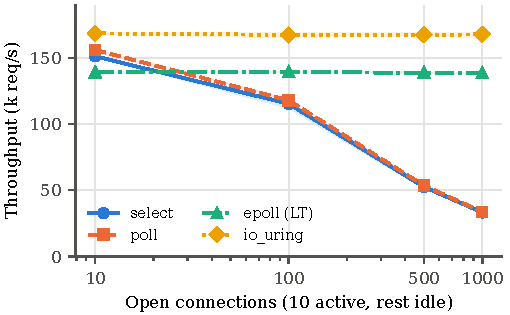
\includegraphics[width=\columnwidth]{figures/idle_scaling.pdf}
\caption{Echo throughput with 10 active clients and an increasing number of idle connections (closed loop, median and min--max of 5 runs).}
\label{fig:idle}
\end{figure}

Fig.~\ref{fig:idle} keeps 10 clients busy and adds idle connections. \code{select} falls from 151.2 to 33.2\,\krps{} and \code{poll} from 156.0 to 33.6\,\krps{} at 1000 descriptors, a 78\% loss, and their CPU per request rises from about 6.5 to 30\us. The system calls per message stay at 3.3, so the extra cost is \emph{inside} each call: the kernel copies the interest list and calls every socket's \code{poll} method twice, ready or not. \code{epoll} (139\,\krps) and \code{io\_uring} (168\,\krps) are flat, because their cost depends on ready events, not registered descriptors. This confirms Banga et al.\ [1]. The crossover is small: already at 100 descriptors, with 90 of them idle, \code{select} and \code{poll} fall below \code{epoll}.

\subsection{Does CPU follow load? (TA's io\_uring question)}
\begin{figure}[t]
\centering
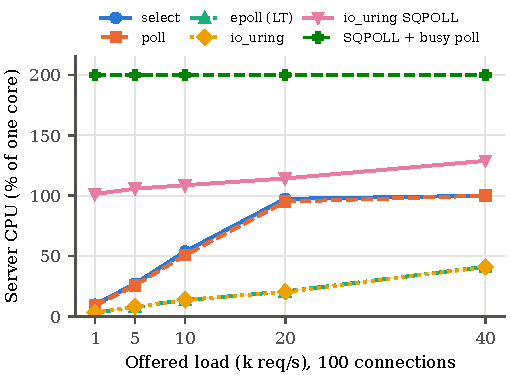
\includegraphics[width=\columnwidth]{figures/rate_sweep_cpu.pdf}
\caption{Server CPU against a paced offered load (echo 64\,B, 100 connections). Plain io\_uring and epoll overlap.}
\label{fig:rate}
\end{figure}

In closed-loop runs every engine shows about 100\% CPU because the client sends as fast as possible; this is what made \code{io\_uring} look like ``90\% CPU at any load''. Fig.~\ref{fig:rate} instead fixes the offered rate. \textbf{Plain \code{io\_uring}'s CPU follows load}, from 3.4\% at 1k\,req/s to 40.9\% at 40k, the same as \code{epoll} (2.8\% to 41.1\%). It sleeps in \code{io\_uring\_enter} when there is nothing to do, with one voluntary context switch per request. Only \textbf{SQPOLL} stays above one core at every load (101\% at 1k\,req/s, 129\% at 40k), because its kernel thread polls the SQ and sleeps only after 100\,ms with no work, which never happens at these rates. With busy completion polling as well, it uses exactly 200\% (two cores) at every load, for the lowest latency of all (p50 14.8\us{} at 40k\,req/s, against 17.0\us{} for plain \code{io\_uring}).

The figure also shows a second cost of scanning. Under light paced load each wakeup finds about one ready socket, so \code{select} and \code{poll} scan all 100 descriptors \emph{per request}: they cost 48--54\us{} per request against 10--16\us{} for \code{epoll} and \code{io\_uring}, saturate one core at about 20k\,req/s, and have three times the median latency at 40k\,req/s (54\us{} against 18\us). In closed loop the same scan was amortised over about 33 requests (Table~\ref{tab:echo}), so \emph{how bursty the load is} decides whether the scan matters.

\subsection{Bulk transfer: upload, download and buffer size}
\begin{table}[t]
\caption{Bulk transfer, 1\,MiB requests, 10 connections, 4\,KiB buffer}
\label{tab:bulk}
\centering\small
\begin{tabular}{@{}lrrrrrr@{}}
\toprule
 & \multicolumn{3}{c}{Upload (read-heavy)} & \multicolumn{3}{c}{Download (write-heavy)}\\
\cmidrule(lr){2-4}\cmidrule(l){5-7}
Engine & MiB/s & CPU/MiB & sc/MiB & MiB/s & CPU/MiB & sc/MiB\\
\midrule
select    & 2681 & 373\us & 292 & 587 & 1705\us & 283\\
poll      & 2849 & 351\us & 291 & 612 & 1634\us & 283\\
epoll LT  & 2764 & 362\us & 293 & 592 & 1688\us & 285\\
io\_uring & \textbf{3097} & \textbf{323\us} & 27 & 609 & 1640\us & 26\\
\bottomrule
\end{tabular}
\end{table}

Table~\ref{tab:bulk} compares the two directions. On upload, \code{io\_uring} is 9--15\% faster and needs 27 kernel entries per MiB instead of about 292, but the CPU per MiB falls by only 8--13\%: almost all of it is kernel time copying data, which every engine pays. On download all engines are within 5\%. Download costs about 4.6$\times$ more CPU per MiB than upload because on loopback the \emph{sender's} CPU also runs the receiver's network processing: we counted 256 NET\_RX softirqs per 1\,MiB request on the server core, one per 4\,KiB segment sent. This is a property of loopback, and it is why we account softirqs separately from the process's own CPU time.

The server buffer size matters far more than the engine. With 64\,KiB instead of 4\,KiB buffers, download rises from 592 to 4519\,MiB/s (7.6$\times$, \code{select}) and upload from 2679 to 10015\,MiB/s, because each system call moves 16 times more data (\code{select}: 283 to 19 syscalls per MiB). At 64\,KiB the engines are within 5\% of each other (download 4330--4519, upload 10015--10254\,MiB/s).

\subsection{Level- versus edge-triggered epoll}
\begin{table}[t]
\caption{epoll modes (closed loop, median of 5)}
\label{tab:epoll}
\centering\small
\begin{tabular}{@{}lrrrrr@{}}
\toprule
 & \multicolumn{3}{c}{echo 64\,B, 100 conns} & \multicolumn{2}{c}{download, 10 conns}\\
\cmidrule(lr){2-4}\cmidrule(l){5-6}
Mode & \krps & sc/msg & ctl/msg & MiB/s & waits/MiB\\
\midrule
LT (default) & 141.2 & 5.03 & 2.00 & 602 & 25.7\\
LT-direct    & \textbf{161.7} & 3.02 & 0.00 & 605 & 25.6\\
ET           & 154.5 & 4.01 & 0.00 & \textbf{685} & 0.1\\
\bottomrule
\end{tabular}
\end{table}

Table~\ref{tab:epoll} answers the TA's LT/ET question. For small echo messages the cost that matters is \code{epoll\_ctl}: both LT-direct and ET avoid it, and LT-direct is fastest. ET pays one extra \code{recv} per request, the one that returns \code{EAGAIN}, which ET requires to be sure the socket is drained. For downloads ET wins by 14\%: one edge notification is followed by sends until the socket buffer is full, so it needs 0.1 waits per MiB instead of 25.7. LT reports the socket again after every 4\,KiB send. The best mode therefore depends on the application: LT-direct for request--response, ET for bulk writes.

\subsection{io\_uring SQPOLL under full load}
\begin{table}[t]
\caption{io\_uring modes, echo 64\,B, closed loop}
\label{tab:sqpoll}
\centering\footnotesize
\begin{tabular}{@{}lrrrrrr@{}}
\toprule
 & \multicolumn{3}{c}{10 connections} & \multicolumn{3}{c}{500 connections}\\
\cmidrule(lr){2-4}\cmidrule(l){5-7}
Mode & \krps & CPU\% & ent./msg & \krps & CPU\% & ent./msg\\
\midrule
plain        & \textbf{168.2} & 100 & 0.30 & \textbf{169.6} & 100 & 0.01\\
SQPOLL       & 145.9 & 112 & 0.30 & 160.5 & 200 & 0.00\\
SQPOLL+busy  & 167.5 & 200 & 0.00 & 161.8 & 200 & 0.00\\
\bottomrule
\end{tabular}
\end{table}

Table~\ref{tab:sqpoll} shows that SQPOLL does not raise throughput on this machine. Plain \code{io\_uring} already needs very few kernel entries per message under load (0.01 at 500 connections), so there is little left for SQPOLL to remove, while the extra thread doubles the CPU and adds hand-off latency between the two cores. At 10 connections, plain SQPOLL is 13\% slower because the application still sleeps in the kernel waiting for completions (0.30 entries per message) and must also wake the SQ thread. SQPOLL is worth its extra core only when the lowest latency matters more than CPU (Fig.~\ref{fig:rate}), as [7] concluded.

Paced SQPOLL also had a heavier tail: its median p99 at 20k--40k\,req/s was 1.1--1.2\,ms, against 21--29\us{} for the other \code{io\_uring} modes. Across these runs, p99 correlates at 0.96 with the time our application thread spent waiting in the run queue on CPU~0, which is also used by other system tasks. When that CPU is briefly taken, the SQ thread on another core keeps polling but the completions wait. The tail is scheduler interference on a shared core, not \code{io\_uring} itself, and our 10\,ms spike sampling found the same cause for the rare spikes in other engines.

\subsection{Streaming, memory-heavy service and UDP}
\begin{table}[t]
\caption{Stream, memory and UDP (median of 5)}
\label{tab:misc}
\centering\footnotesize
\begin{tabular}{@{}lrrrr@{}}
\toprule
 & select & poll & epoll & io\_uring \\
\midrule
\multicolumn{5}{@{}l}{\emph{Stream: 100 conns $\times$ 30 frames/s of 64\,KiB (187.5\,MiB/s)}}\\
Server CPU \%      & 96.7 & 94.4 & 30.2 & \textbf{29.4}\\
p50 latency (\us)  & 338  & 326  & 109  & \textbf{107}\\
\midrule
\multicolumn{5}{@{}l}{\emph{Memory: 500 conns, 256\,KiB per client, 4\,KiB writes}}\\
\krps              & 148.4 & 149.4 & 125.9 & \textbf{149.9}\\
Peak RSS (MiB)     & 130.5 & 130.6 & 130.5 & 130.8\\
\midrule
\multicolumn{5}{@{}l}{\emph{UDP echo, 100 flows, one socket (\krps); io\_uring at depth 1 / 32}}\\
64\,B   & \textbf{242.0} & 241.6 & 234.3 & 199.2 / 237.2\\
1400\,B & \textbf{232.9} & 232.8 & 226.4 & 192.2 / 225.1\\
4096\,B & 175.9 & 175.3 & 173.0 & 176.9 / \textbf{201.1}\\
\bottomrule
\end{tabular}
\end{table}

\textbf{Streaming} (Table~\ref{tab:misc}) is paced, so it behaves like the rate sweep: each 64\,KiB frame is sent in 16 pieces of 4\,KiB, about 17 waits per frame, and each \code{select}/\code{poll} wait scans all 100 descriptors. They therefore need 3.2$\times$ the CPU of \code{epoll}/\code{io\_uring} (322 against 100\us{} per frame) for the same data, and their median frame latency is three times higher.

\textbf{Memory-heavy service.} Each of 500 clients holds a resident 256\,KiB buffer (130\,MiB peak RSS for every engine, against 1.8\,MiB for echo). The engine ranking is the same as for echo: \code{io\_uring}, \code{poll} and \code{select} at 148--150\,\krps{} and LT \code{epoll} 15\% lower because of \code{epoll\_ctl}. Memory per client is a property of the application, not of the multiplexing mechanism: with echo, every engine's server stays at 1.8--2.5\,MiB.

\textbf{UDP.} A UDP server uses one socket for all clients, so there is no $O(N)$ scan and \code{select} and \code{poll} are as fast as \code{epoll}. \code{io\_uring} with one outstanding receive (depth 1) is 18\% \emph{slower} for small datagrams: each datagram needs two kernel entries (submit the receive, then the send) and nothing is batched. With 32 receives outstanding it needs 0.06 entries per datagram and matches the readiness engines; for 4096\,B datagrams it is 14\% faster. As with TCP, \code{io\_uring} helps only when it can batch.

\subsection{Multiple event loops}
\begin{figure}[t]
\centering
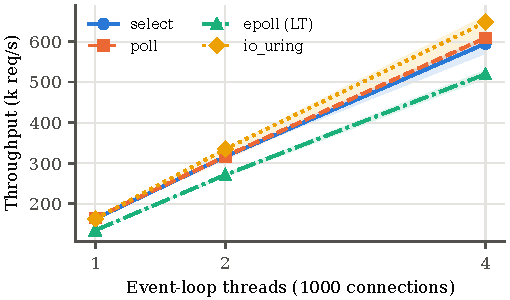
\includegraphics[width=\columnwidth]{figures/multithread.pdf}
\caption{Echo 64\,B with 1000 connections spread over 1, 2 and 4 independent event loops (\code{SO\_REUSEPORT}), one per physical core.}
\label{fig:mt}
\end{figure}

Fig.~\ref{fig:mt} shows near-linear scaling for every engine, because the loops share nothing: four loops give 3.65$\times$ (\code{select}), 3.70$\times$ (\code{poll}), 3.87$\times$ (\code{epoll}) and 3.98$\times$ (\code{io\_uring}). \code{io\_uring} reaches 648\,\krps{} with four loops. The ranking with one loop is preserved, so the mechanism's per-request cost still matters after scaling out.

\subsection{Interrupts and wakeups}
On loopback no device interrupts reached the server core in any run; the network work appears as softirqs instead. Each echo request causes one NET\_RX softirq on the server core (for the reply it sends), and each 1\,MiB download causes 256. In closed loop no engine sleeps (0 voluntary context switches per message), because work is always waiting. In paced mode every engine that is not saturated sleeps and is woken once per request; busy-polling SQPOLL never sleeps.

\subsection{Summary of findings}
\begin{table}[t]
\caption{Which mechanism to use}
\label{tab:summary}
\centering\small
\begin{tabularx}{\columnwidth}{@{}>{\raggedright\arraybackslash}p{27mm}X@{}}
\toprule
Situation & Best choice and reason\\
\midrule
All connections busy, small messages & \code{io\_uring} (+6--7\%); \code{select}/\code{poll} next; LT \code{epoll} worst (2 \code{epoll\_ctl}/req)\\
Many idle connections & \code{epoll} or \code{io\_uring}; \code{select}/\code{poll} lose 78\% at 1000 fds\\
Light or paced load & \code{epoll}/\code{io\_uring}; \code{select}/\code{poll} scan all fds per request\\
Bulk transfer & Buffer size dominates (up to 7.6$\times$); engines within 5\% at 64\,KiB\\
Bulk writes with epoll & ET (+14\%)\\
UDP (one socket) & Any readiness engine; \code{io\_uring} only with deep queues\\
Lowest latency, spare cores & SQPOLL + busy polling (2 cores at any load)\\
\bottomrule
\end{tabularx}
\end{table}

Table~\ref{tab:summary} summarises the results. The literature's predictions held: with all connections active the readiness mechanisms are close [3]; with idle connections \code{select} and \code{poll} degrade and \code{epoll} does not [1]; \code{io\_uring}'s gain is modest [7]. We also found that under light load the scan cost appears per request, that \code{epoll}'s default LT mode is held back by \code{epoll\_ctl}, and that UDP removes the scanning difference.

%======================================================================
\section{Summary}
We asked which Linux I/O multiplexing mechanism a single-threaded server should use, and found that the answer depends on the application and the load. Using one framework in which four engines share all application code, we measured six applications over TCP and UDP in 1140 validated runs and explained each result by system calls, scanning, wakeups, softirqs and CPU. \code{select} and \code{poll} are competitive when every connection is busy, but their per-call scan of all descriptors costs up to 78\% of throughput with idle connections and dominates under light load. \code{epoll} is flat in the number of descriptors but its default level-triggered use pays two \code{epoll\_ctl} calls per request, which the LT-direct and ET modes remove. \code{io\_uring} is fastest wherever operations can be batched (6--15\%), gains nothing without batching, and its CPU follows load; only SQPOLL trades a permanently busy core for latency.

\textbf{Limitations.} All results are on loopback, where receive processing runs on the sender's CPU, and on one laptop whose CPU~0 is shared with system tasks; upload and download use memory patterns instead of files; \code{io\_uring} was limited to liburing 2.1 (no multishot receive, no registered buffers).
\textbf{Future work.} Repeat on two machines with a real NIC and interrupt affinity; add multishot receive, registered buffers and zero-copy send; test thread-per-connection and shared-queue multithreaded designs; and run real file I/O.

%======================================================================
\section{Reproducibility}
\textbf{Repository:} \url{https://github.com/devvrat-hans/CS331-T016-ScalableNetworkIO}. The engines are in \code{code/select}, \code{code/poll}, \code{code/epoll} and \code{code/io\_uring}; the framework, plugins, load generator and scripts in \code{code/benchmark}.

\textbf{Requirements:} Linux $\geq$ 5.15 with \code{io\_uring} enabled, gcc, make, \code{liburing-dev}, Python 3, \code{strace}, \code{iproute2}.

\textbf{Steps:}
\begin{enumerate}
\item Prepare the machine (mains power, Wi-Fi off):\\[1pt]
{\footnotesize\ttfamily sudo apt install build-essential \textbackslash\\
\hspace*{2em}liburing-dev strace iproute2 python3\\
sudo cpupower frequency-set -g performance\\
sudo sysctl -w net.core.rmem\_max=8388608\\
sudo sysctl -w net.core.wmem\_max=8388608}
\item Build and run everything: \code{cd code/benchmark \&\& ./run\_all.sh}. This checks the environment, builds with \code{make}, runs the correctness tests, the counter check against \code{strace}, the client cross-check, all benchmark suites (about 5 hours), the analysis and the latency-spike diagnosis.
\item Individual parts:\\[1pt]
{\footnotesize\ttfamily python3 correctness.py OUT\\
python3 experiments.py run \textbackslash\\
\hspace*{2em}-{}-suites idle-scaling -{}-out OUT\\
python3 experiments.py analyze \textbackslash\\
\hspace*{2em}-{}-input OUT -{}-out REPORT}
\item Results: \code{results/final/report/report.md} (tables), \code{aggregates.csv} (all medians, min and max) and one folder per run with the exact server and client command lines and their JSON outputs.
\end{enumerate}

%======================================================================
\begin{thebibliography}{9}
\bibitem{banga} G. Banga, J. C. Mogul, and P. Druschel, ``A scalable and explicit event delivery mechanism for UNIX,'' in \emph{Proc. USENIX Annu. Tech. Conf.}, Monterey, CA, USA, 1999, pp. 253--266.
\bibitem{provos} N. Provos and C. Lever, ``Scalable network I/O in Linux,'' in \emph{Proc. USENIX Annu. Tech. Conf., FREENIX Track}, San Diego, CA, USA, 2000.
\bibitem{gammo} L. Gammo, T. Brecht, A. Shukla, and D. Pariag, ``Comparing and evaluating epoll, select, and poll event mechanisms,'' in \emph{Proc. Ottawa Linux Symp.}, Ottawa, Canada, 2004, pp. 215--226.
\bibitem{flexsc} L. Soares and M. Stumm, ``FlexSC: Flexible system call scheduling with exception-less system calls,'' in \emph{Proc. USENIX OSDI}, Vancouver, Canada, 2010.
\bibitem{schroeder} B. Schroeder, A. Wierman, and M. Harchol-Balter, ``Open versus closed: A cautionary tale,'' in \emph{Proc. USENIX NSDI}, San Jose, CA, USA, 2006, pp. 239--252.
\bibitem{didona} D. Didona, J. Pfefferle, N. Ioannou, B. Metzler, and A. Trivedi, ``Understanding modern storage APIs: A systematic study of libaio, SPDK, and io\_uring,'' in \emph{Proc. ACM SYSTOR}, Haifa, Israel, 2022, pp. 120--127, doi: 10.1145/3534056.3534945.
\bibitem{dbms} ``io\_uring for high-performance DBMSs: When and how to use it,'' arXiv:2512.04859, 2025.
\bibitem{axboe} J. Axboe, ``Efficient IO with io\_uring,'' 2019. [Online]. Available: \url{https://kernel.dk/io_uring.pdf}
\end{thebibliography}

%======================================================================
\clearpage
\onecolumn
\appendices
\renewcommand{\arraystretch}{1.35}
\newcommand{\hdr}{\rowcolor[gray]{0.86}}

\section*{Appendix A: Team Work Distribution and Member Rating}
\subsection*{A.1 Work Distribution}
\begin{itemize}
\item Ratings are agreed by the whole team and are unique: no two members received the same rating (no ties).
\item Scale: 1--10 (10 = highest contribution). With six members, six different values are used (10 to 5).
\end{itemize}

\vspace{3mm}
\noindent
{\small
\begin{tabularx}{\textwidth}{|>{\centering\arraybackslash}p{6mm}|>{\raggedright\arraybackslash}p{34mm}|>{\centering\arraybackslash}p{17mm}|>{\raggedright\arraybackslash}X|>{\centering\arraybackslash}p{19mm}|}
\hline
\hdr \textbf{\#} & \centering\textbf{Member Name} & \textbf{Roll No.} & \centering\textbf{Tasks Done} & \textbf{Rating (1--10, unique)}\\
\hline
1 & Kale Parth Hemant    & 24110242 & \code{select} engine (\code{select\_server.c}): descriptor table, read/write set construction, \code{FD\_SETSIZE} guard, TCP and UDP loops. & 9\\
\hline
2 & Devvrat Hans         & 23110094 & \code{poll} engine (\code{poll\_server.c}): parallel \code{pollfd}/client arrays, per-iteration interest rebuild, TCP and UDP loops. & 6\\
\hline
3 & Patil Nachiket Kiran & 24110250 & \code{epoll} engine (\code{epoll\_server.c}) in level-triggered, edge-triggered and LT-direct modes; ran all experiments on his laptop (the testbed). & 7\\
\hline
4 & Niraj Kumar          & 24110222 & \code{io\_uring} engine (\code{io\_uring\_server.c}): plain, SQPOLL and busy-poll modes, completion-queue sizing, UDP receive depth, shutdown and cancellation. & 5\\
\hline
5 & Chirag Agarwalla     & 24110093 & Benchmarking: shared framework and plugins, C load generator, experiment runner and analysis, correctness tests, counter and client cross-checks. & 10\\
\hline
6 & Nityanand Karmali    & 24110226 & Report, presentation slides and literature review. & 8\\
\hline
\end{tabularx}}

\clearpage
\section*{Appendix B: AI Usage Details}
\subsection*{B.1 Prompts}
The links to the prompts and chat logs for the most significant uses listed in the table are given below it.

\vspace{3mm}
\noindent
{\small
\begin{tabularx}{\textwidth}{|>{\centering\arraybackslash}p{6mm}|>{\raggedright\arraybackslash}p{62mm}|>{\raggedright\arraybackslash}X|}
\hline
\hdr \textbf{\#} & \centering\textbf{AI Tool} & \centering\arraybackslash\textbf{Purpose}\\
\hline
1 & Claude, Gemini (Kale Parth Hemant) & Understanding the project and the four mechanisms; designing and implementing the \code{select} server.\\
\hline
2 & Freebuff / Codebuff with DeepSeek V4 Flash (Devvrat Hans) & Understanding how \code{poll} differs from \code{select} inside the kernel; generating the \code{poll} server from his specification; adding comments; writing the component README.\\
\hline
3 & Claude (Patil Nachiket Kiran) & Evolving his first \code{epoll} echo server into the project's \code{epoll} engine with echo, upload and download workloads; planning the architecture, measurement matrix and metrics (project phases 4--6); a phase-by-phase review of the final \code{epoll} engine (LT, LT-direct and ET paths, UDP, risks and counters).\\
\hline
4 & ChatGPT (Niraj Kumar): chats ``Explain Sockets And I O'' and ``Clarify Io Uring Project'' & Understanding sockets, file descriptors and blocking versus non-blocking I/O; clarifying the \code{io\_uring} design and the Phase~2 framework.\\
\hline
5 & ChatGPT, Gemini (Chirag Agarwalla) & Building the benchmarking framework; reviewing the engines against the test bench; background on the theory and expected behaviour of the four mechanisms.\\
\hline
6 & Claude Code with Claude Opus 5.5 (Nityanand Karmali): chat ``Network I/O server benchmarking fixes'' & Reviewing the code and first results against the TA feedback; fixing and extending the framework and experiments; analysing the final results; checking review comments on the engines; drafting this report and the presentation slides.\\
\hline
\end{tabularx}}

\vspace{5mm}
\noindent Relevant prompt queries and response \code{.md} files are shared on GitHub in the \code{AI\_Usage} folder (\url{https://github.com/devvrat-hans/CS331-T016-ScalableNetworkIO/tree/main/AI_Usage}):
\begin{enumerate}\raggedright
\item Kale Parth Hemant (\code{AI\_Usage/select}):\\\url{https://github.com/devvrat-hans/CS331-T016-ScalableNetworkIO/tree/main/AI_Usage/select}\\
Files: \code{claude\_chat.md}, \code{gemini\_chat.pdf}
\item Devvrat Hans (\code{AI\_Usage/poll}):\\\url{https://github.com/devvrat-hans/CS331-T016-ScalableNetworkIO/tree/main/AI_Usage/poll}\\
File: \code{ai\_usage\_poll.md}
\item Patil Nachiket Kiran (\code{AI\_Usage/epoll}):\\\url{https://github.com/devvrat-hans/CS331-T016-ScalableNetworkIO/tree/main/AI_Usage/epoll}\\
Claude chats: ``Epoll echo server evolution part 1'', ``Phase 4, 5, and 6 implementation part 2'' and ``Phase 4, 5, and 6 implementation part 3''
\item Niraj Kumar (\code{AI\_Usage/io\_uring}):\\\url{https://github.com/devvrat-hans/CS331-T016-ScalableNetworkIO/tree/main/AI_Usage/io_uring}\\
ChatGPT chats: ``Explain Sockets And I O'' and ``Clarify Io Uring Project''
\item Chirag Agarwalla (\code{AI\_Usage/benchmark}):\\\url{https://github.com/devvrat-hans/CS331-T016-ScalableNetworkIO/tree/main/AI_Usage/benchmark}\\
ChatGPT chats: ``Build Linux IO Benchmarking Framework'' and ``Backend Testing Results''; Gemini chat: ``Linux I/O Multiplexing Mechanisms Compared''
\item Nityanand Karmali (\code{AI\_Used/Report\_PPT}):\\\url{https://github.com/devvrat-hans/CS331-T016-ScalableNetworkIO/blob/dev/nitya/AI_Used/Report_PPT/claude_chat.md}\\
Claude Code chat: ``Network I/O server benchmarking fixes'' (file: \code{claude\_chat.md})
\end{enumerate}

\end{document}
